\documentclass[11pt,a4paper]{article}

% --- Packages ---
\usepackage[utf8]{inputenc} 
\usepackage[T1]{fontenc}    
\usepackage{geometry}       
\geometry{
    a4paper,
    total={170mm,257mm},
    left=25mm,
    top=25mm,
}
\usepackage{graphicx}       
\usepackage{amsmath, amssymb} 
\usepackage{hyperref}       
\hypersetup{                
    colorlinks=true,
    linkcolor=black,
    urlcolor=black,
}
\usepackage{indentfirst}
\usepackage{float}
\usepackage{listings}
\usepackage{xcolor}
\usepackage{tikz}
\usetikzlibrary{arrows.meta, positioning, shapes.geometric}

\lstset{
    basicstyle=\ttfamily\footnotesize,
    commentstyle=\color{green!60!black},
    keywordstyle=\color{blue},
    numbers=left,
    numberstyle=\tiny\color{gray},
    frame=single,
}

% Title and labeling
\title{Image Processing \\ [1ex] \large ECSE 313 Group 16 Lab 5 Report}
\author{Nathaniel Hahn and Donovan Crowley}
\date{\today}

% Body
\begin{document}

\maketitle 

\tableofcontents 
\newpage

\section{Introduction Exercise}
By converting the image pixels from uint8 to double, the provided 'yacht.tif' pixels can be adjusted to invert, negate, and multiply the image.

\begin{figure}[H]
    \centering
    
\includegraphics[width=0.8\textwidth]{../Figure_1.png}
    \caption{Original Yacht Image}
\end{figure}

\begin{figure}[H]
    \centering
    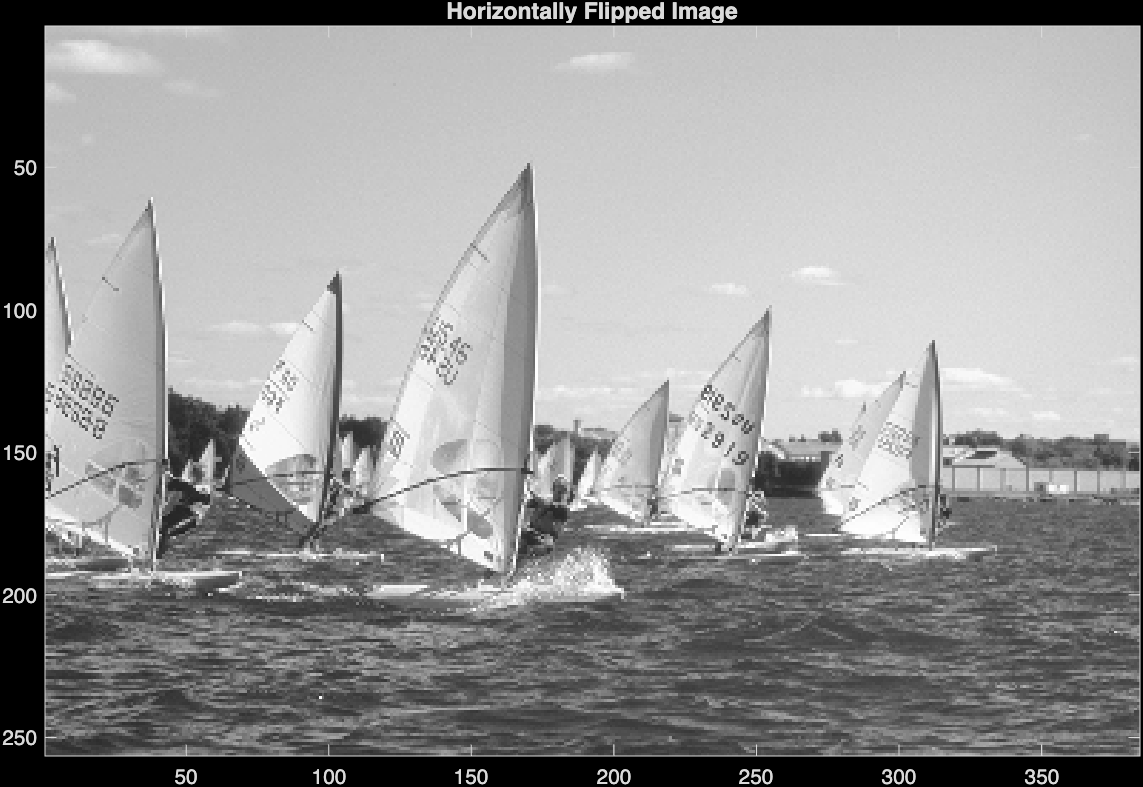
\includegraphics[width=0.8\textwidth]{../Figure_2.png}
    \caption{Horizontally Flipped Yacht Image}
\end{figure}

\begin{figure}[H]
    \centering
    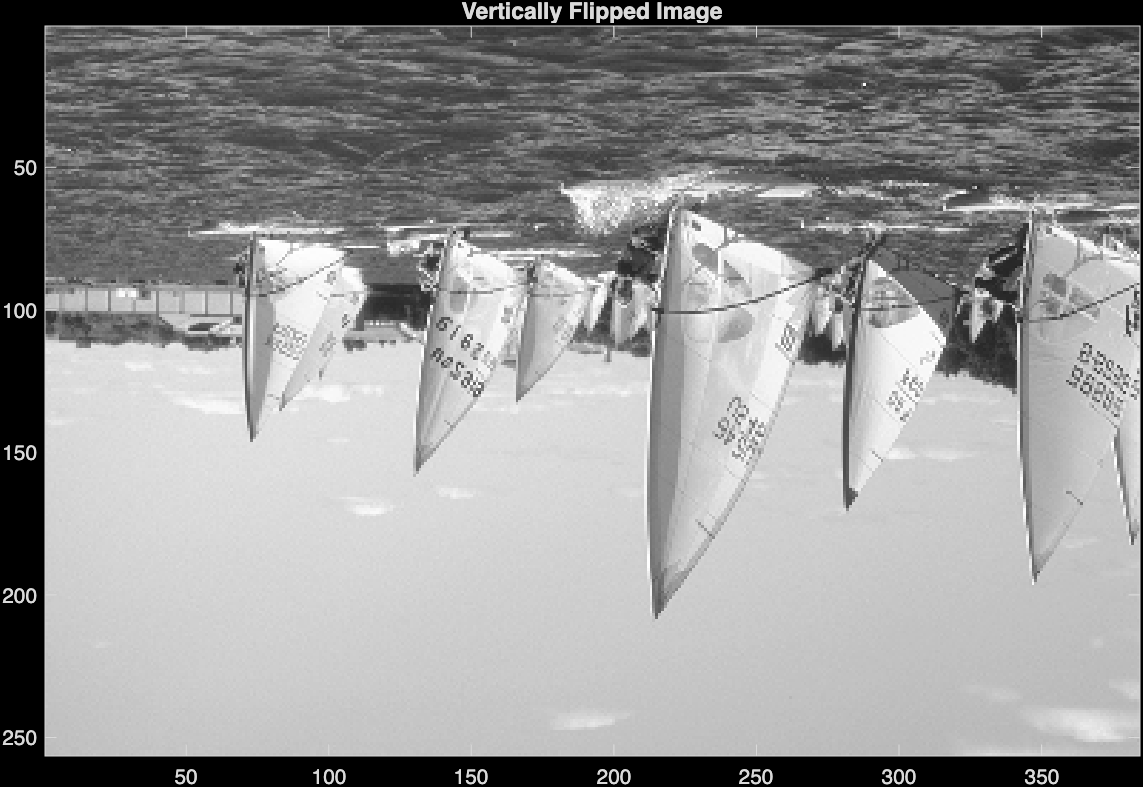
\includegraphics[width=0.8\textwidth]{../Figure_3.png}
    \caption{Vertically Flipped Yacht Image}
\end{figure}

\begin{figure}[H]
    \centering
    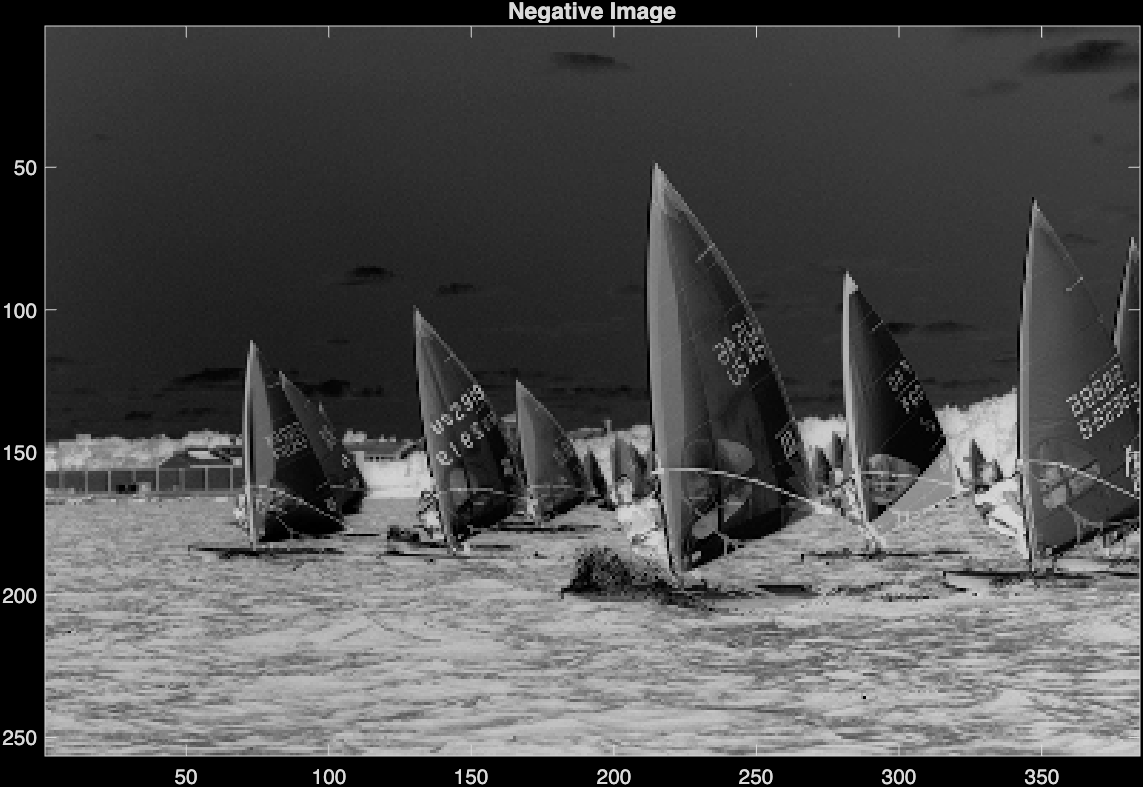
\includegraphics[width=0.8\textwidth]{../Figure_4.png}
    \caption{Negated Yacht Image}
\end{figure}

\begin{figure}[H]
    \centering
    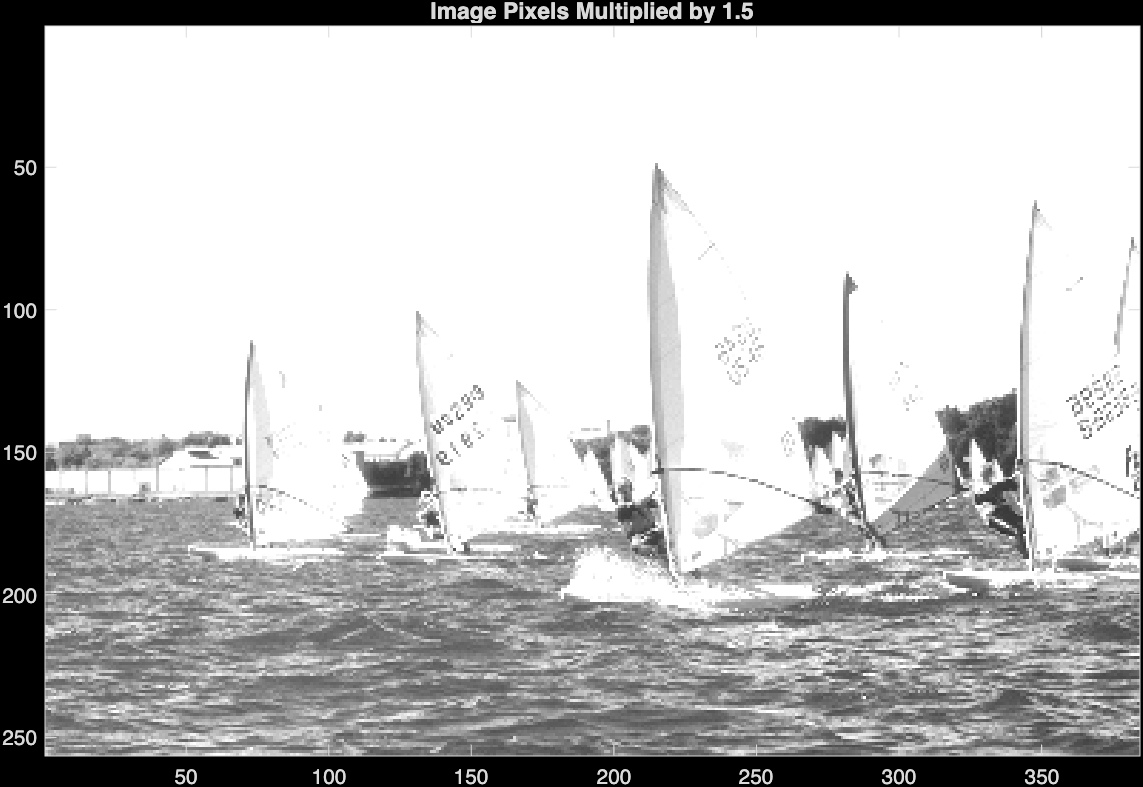
\includegraphics[width=0.8\textwidth]{../Figure_5.png}
    \caption{Yacht Image Pixel Intensities Multiplied by 1.5}
    \label{fig5}
\end{figure}

The effect seen in Fig. \ref{fig5} is the pixel intensities get close to a value of 255 and the image becomes more white. 
The reason for this effect is the pixel intensities are multiplied by a factor of 1.5.
If the pixel intensities were multiplied by a value less than 1, the picture would appear more black as the image intensities would approach 0 or black.
A multiplication of 1 would have no change in the original image.


\section{Histogram of an Image}
\begin{figure}[H]
    \centering
    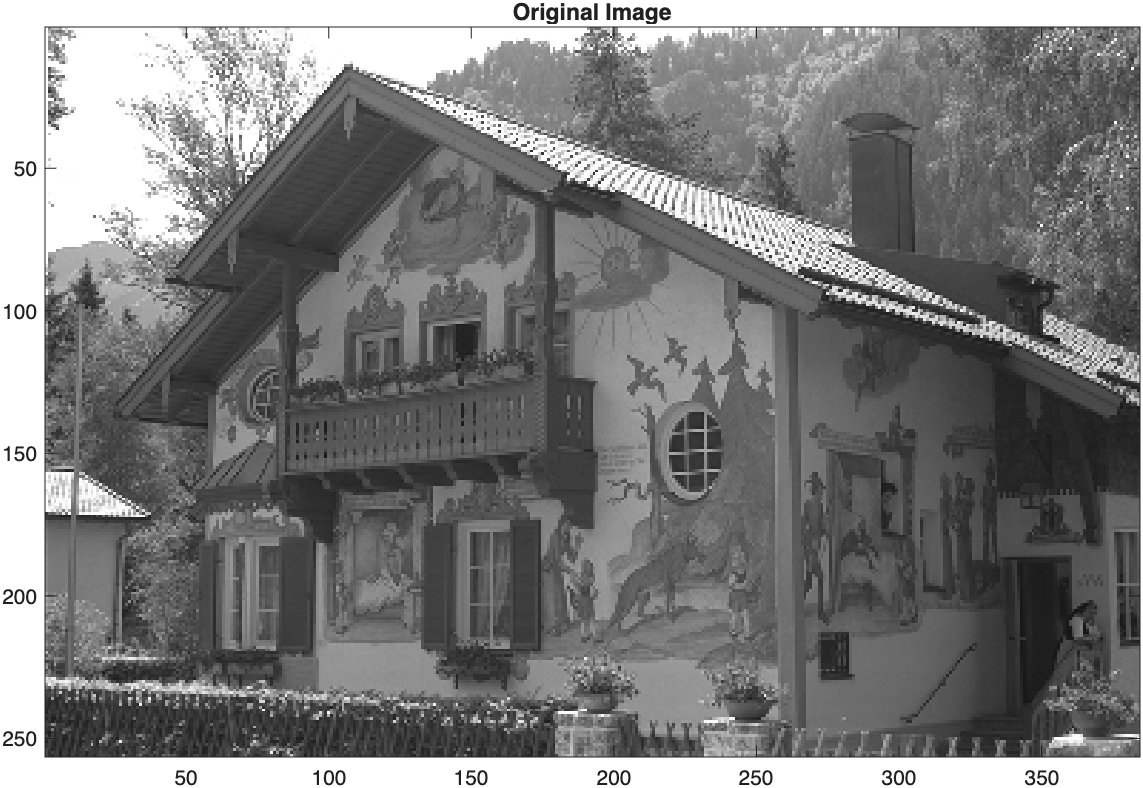
\includegraphics[width=0.8\textwidth]{../Figure_14.png}
    \caption{Original House Image}
\end{figure}


\begin{figure}[H]
    \centering
    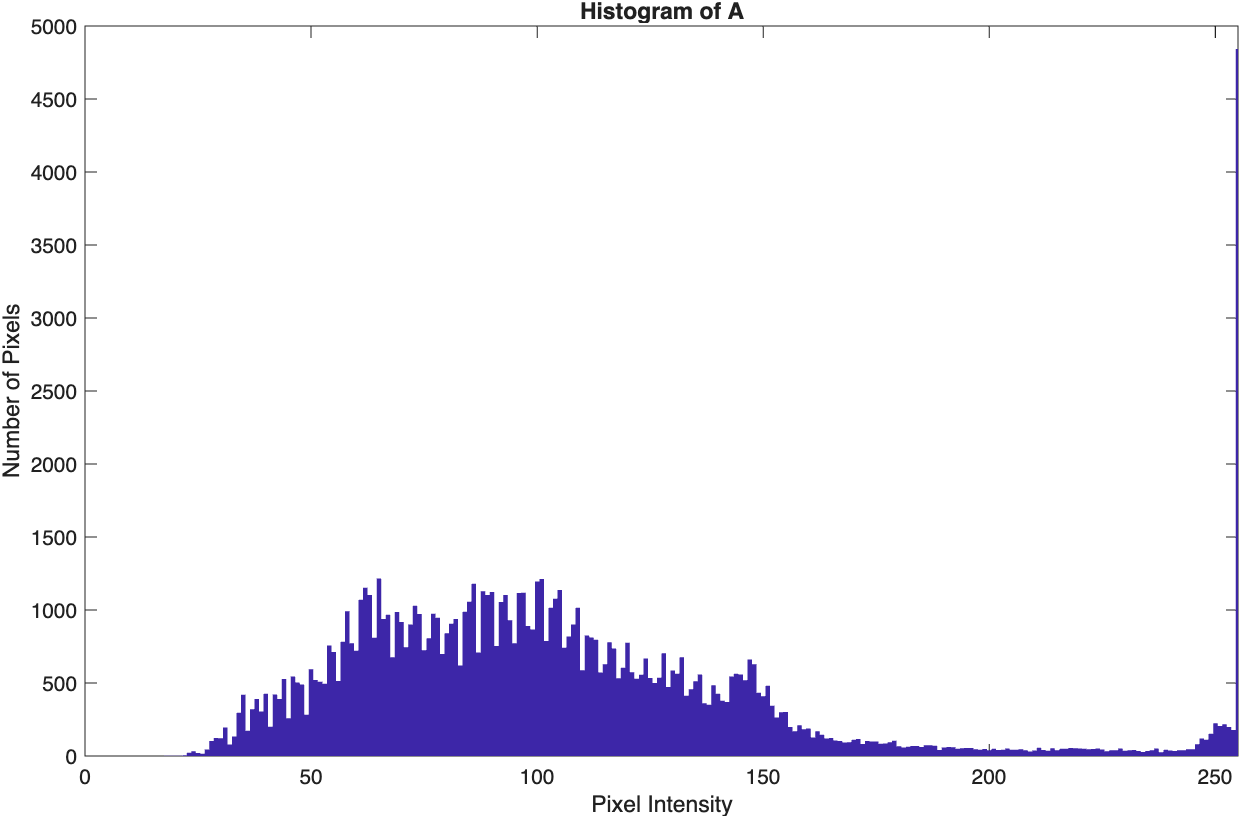
\includegraphics[width=0.8\textwidth]{../Figure_6.png}
    \caption{Histogram of House Image}
    \label{fig6}
\end{figure}

The histogram in Fig. \ref{fig6} has a primary clumped distributions of pixel intensities.
The pixel clump occurs at a range from about 30 to 160 pixel intensities.
This range has a consistent number of pixels at about 750 for each pixel intensity.

Additionally, about 4800 pixels have a pixel intensity of 255 (or black).

\section{Pointwise Transformations}

\lstinputlisting[language=Matlab, title={pointTrans.m}]{../16.3.2/pointTrans.m}

\begin{figure}[H]
    \centering
    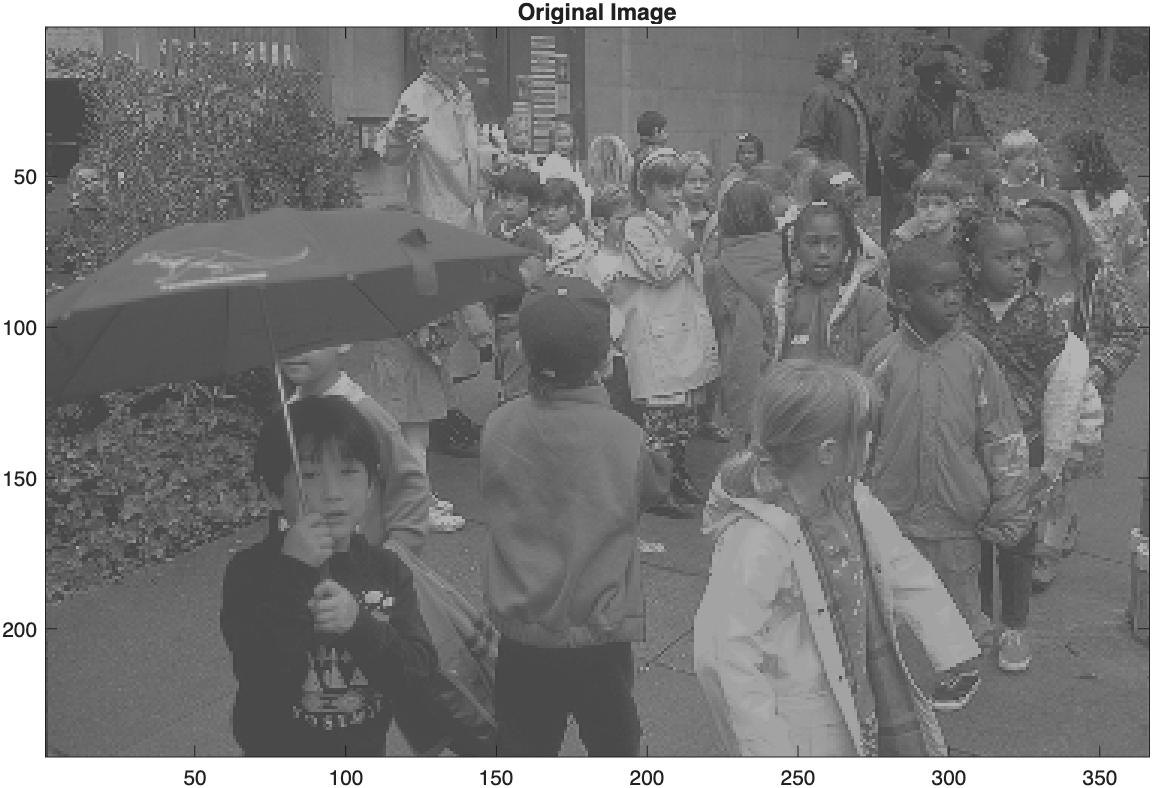
\includegraphics[width=0.8\textwidth]{../Figure_7.png}
    \caption{Original Narrow Image}
    \label{fig7}
\end{figure}

\begin{figure}[H]
    \centering
    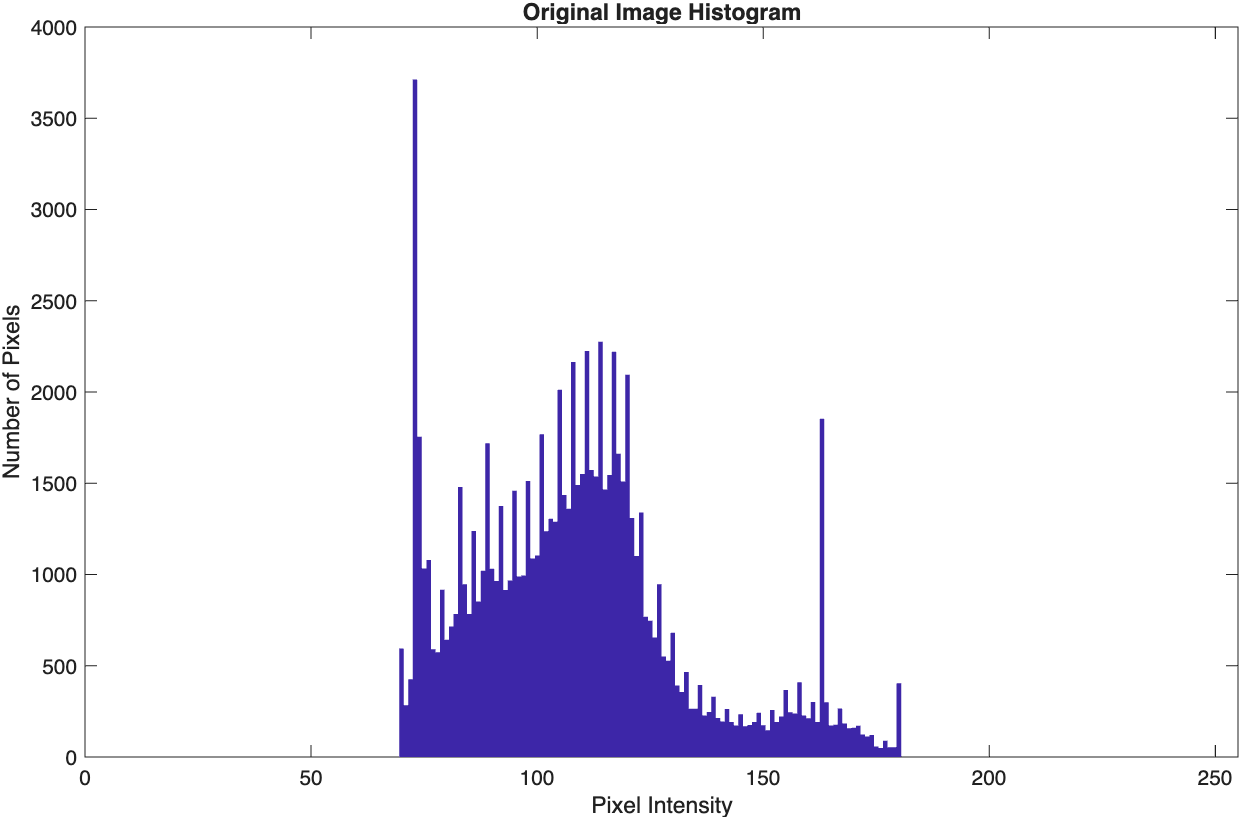
\includegraphics[width=0.8\textwidth]{../Figure_8.png}
    \caption{Histogram of Narrow Image}
    \label{fig8}
\end{figure}

\begin{figure}[H]
    \centering
    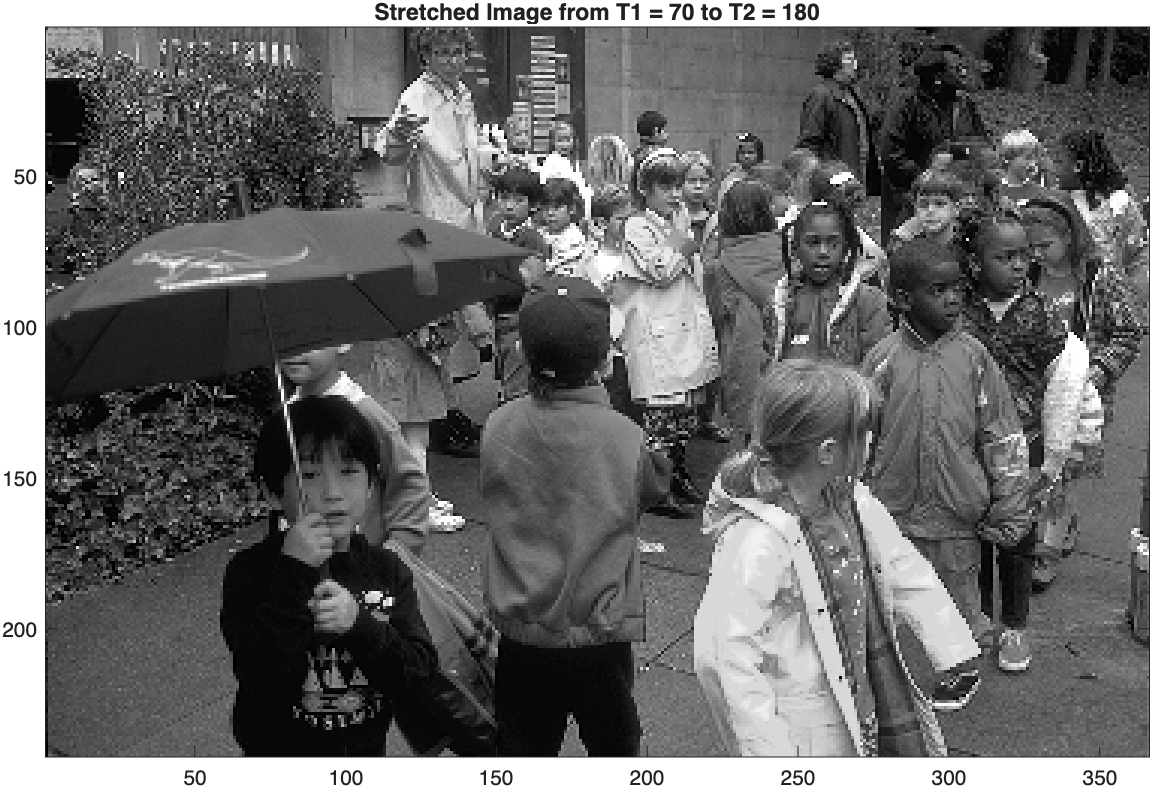
\includegraphics[width=0.8\textwidth]{../Figure_9.png}
    \caption{Stretched Narrow Image}
    \label{fig9}
\end{figure}

\begin{figure}[H]
    \centering
    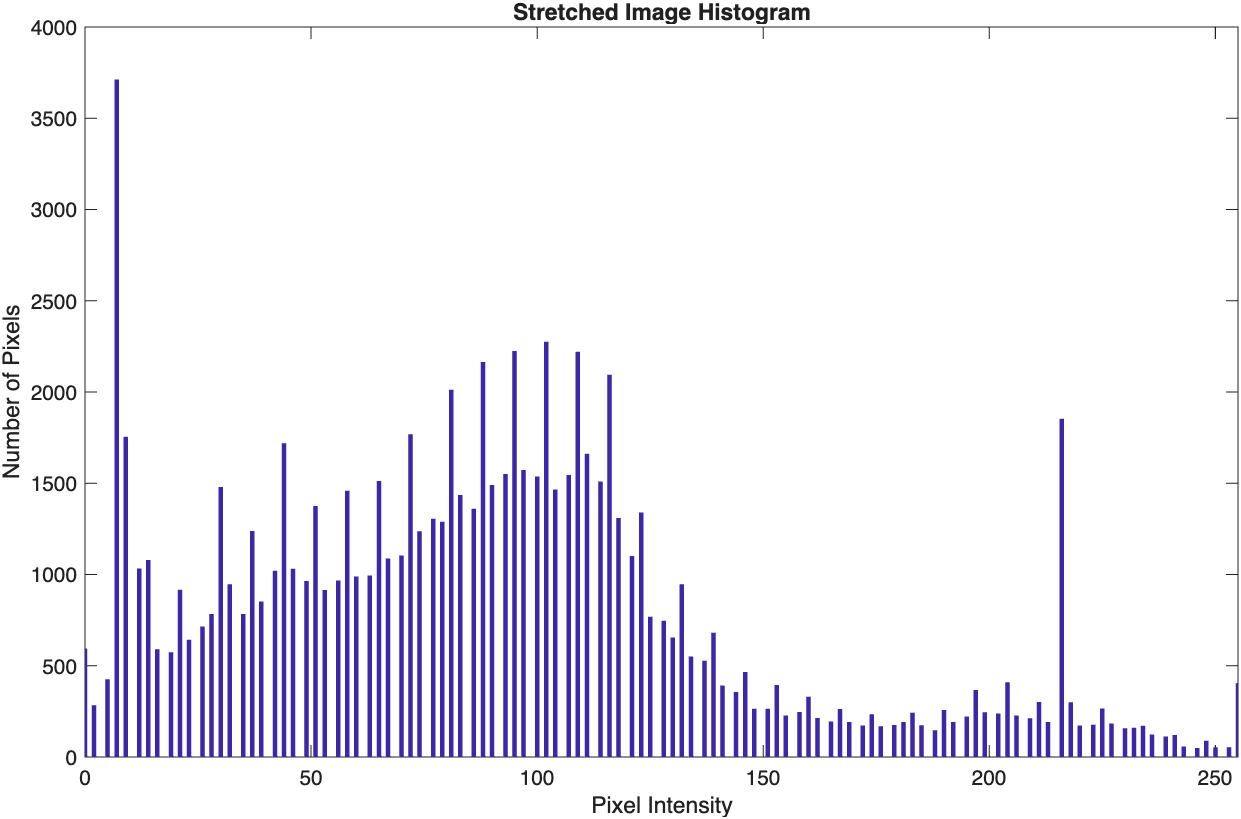
\includegraphics[width=0.8\textwidth]{../Figure_10.png}
    \caption{Histogram of Stretched Narrow Image}
    \label{fig10}
\end{figure}

Stretching an image, as seen in Fig. \ref{fig9}, makes the pixels appear brighter and cleaner as opposed to the original image in Fig. \ref{fig7}. 
However, when looked at closely, Fig. \ref{fig9} is blurry at the outlines of the objects and people due to the stretching effect.
Moreover, while Fig. \ref{fig9} provides a cleaner version than the foggy original version, the stretched image intensifies the individual pixels to make the image more blurry. 

The histogram in Fig. \ref{fig8} is more clumped and confined in a pixel intensity range of about 70 to 180.
The histogram in Fig. \ref{fig10} provides a much more diverse range where the pixel intensities span the entire range.
The zeros in the histogram correspond to the black pixels in the image.

\section{Gamma Correction}
\begin{figure}[H]
    \centering
    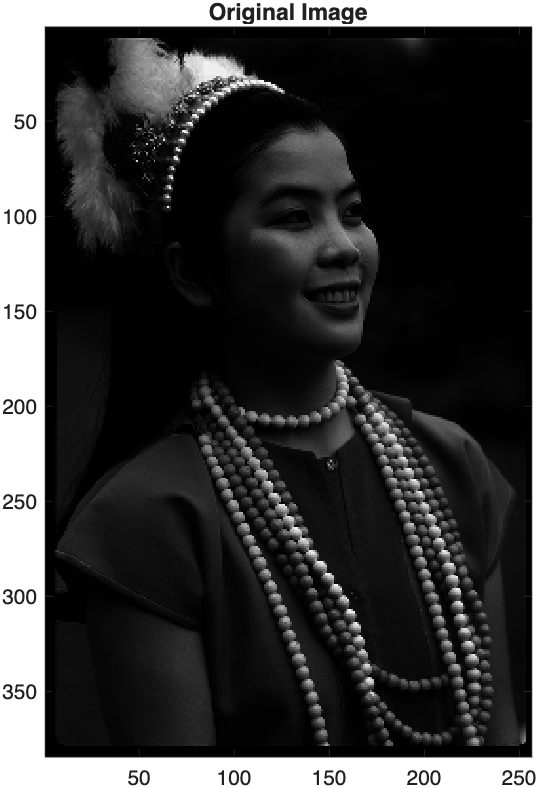
\includegraphics[width=0.8\textwidth]{../Figure_11.png}
    \caption{Original Dark Image}
\end{figure}

\begin{figure}[H]
    \centering
    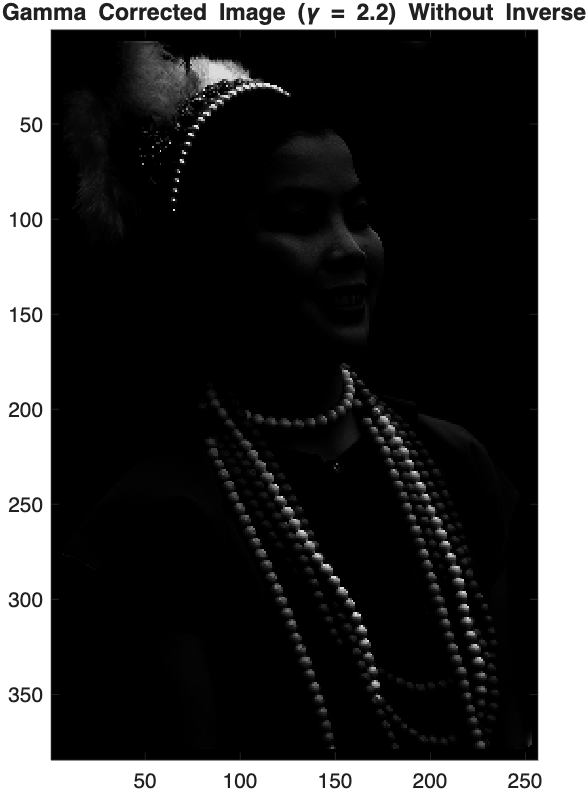
\includegraphics[width=0.8\textwidth]{../Figure_13.png}
    \caption{Original Gamma Corrected Image}
    \label{fig13}
\end{figure}

\begin{figure}[H]
    \centering
    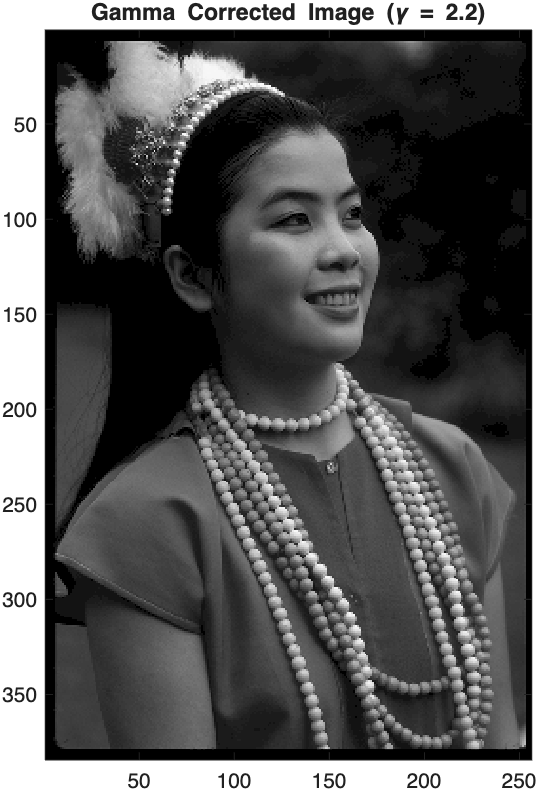
\includegraphics[width=0.8\textwidth]{../Figure_12.png}
    \caption{Inverse Gamma Corrected Image}
    \label{fig12}
\end{figure}

\lstinputlisting[language=Matlab, title={gammCorr.m}]{../16.4/gammCorr.m}

The gamma corrected image as seen in Fig. \ref{fig13} with the original equation given in the problem statement was too dark.
Therefore, we used the inverse as seen in the Matlab script gammCorr.m to produce a better quality image. 
Figure \ref{fig12} shows the inverse gamma corrected image. 
The inverse gamma corrected image is clearer and brighter compared to the original dark version. 

\section{Image Smoothing}

\lstinputlisting[language=Matlab, title={gaussFilter.m}]{../16.5/gaussFilter.m}

\lstinputlisting[language=Matlab, title={medianFilter.m}]{../16.5/medianFilter.m}

\begin{figure}[H]
    \centering
    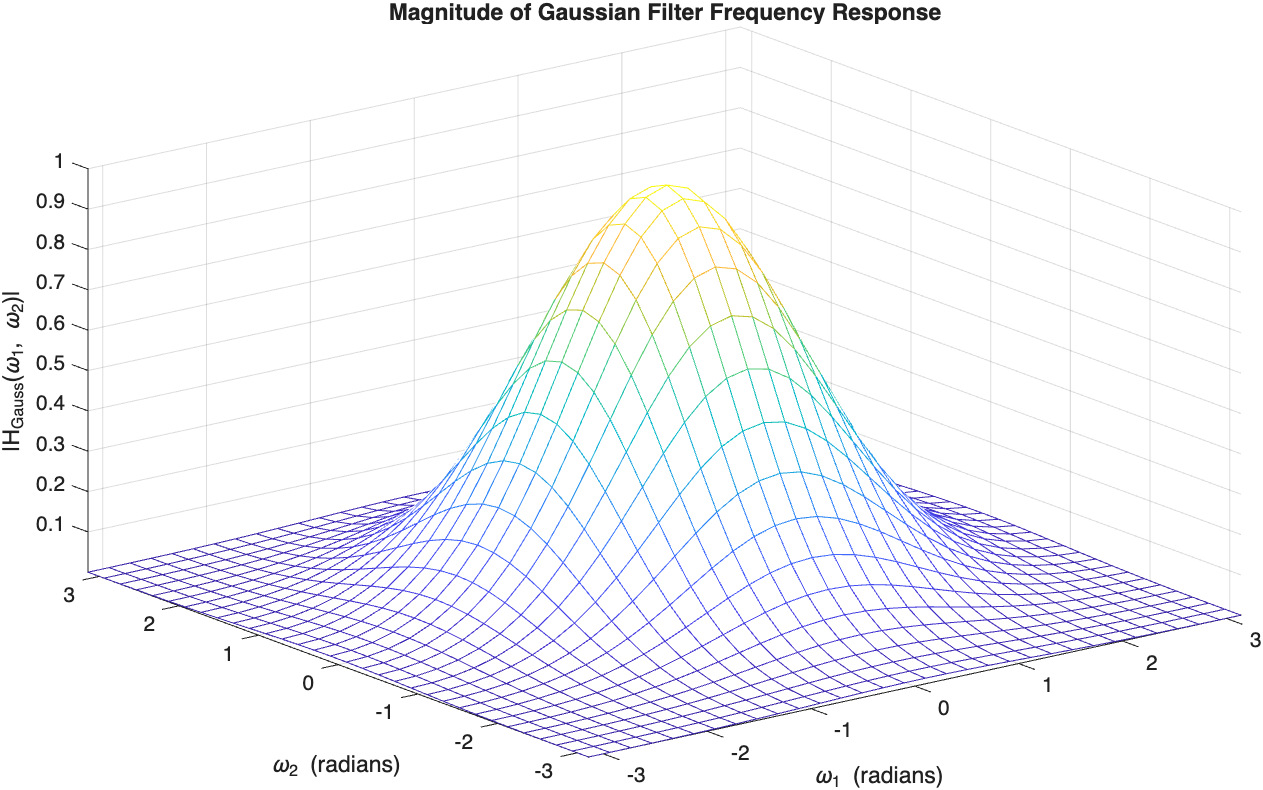
\includegraphics[width=0.8\textwidth]{../Figure_15.png}
    \caption{Magnitude of the Frequency Response of the Gaussian Filter}
\end{figure}

\begin{figure}[H]
    \centering
    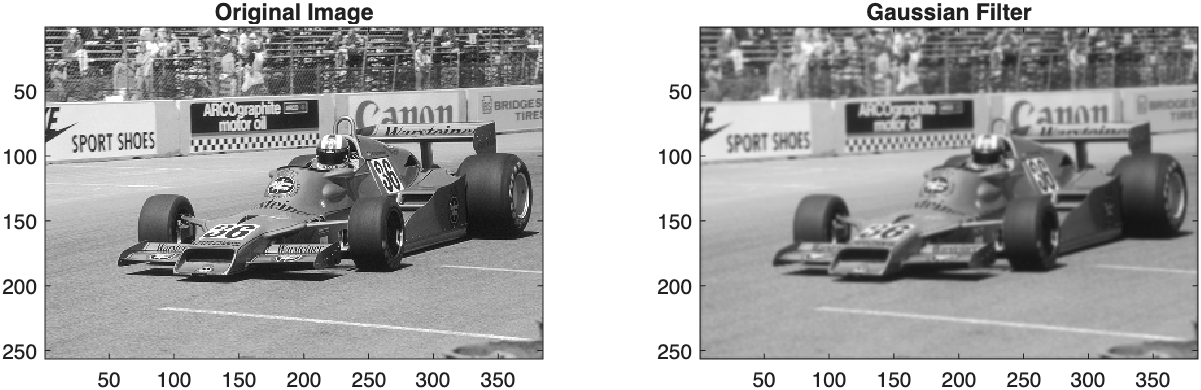
\includegraphics[width=0.8\textwidth]{../Figure_16.png}
    \caption{Original Race Image and Gaussian Filter}
\end{figure}

\begin{figure}[H]
    \centering
    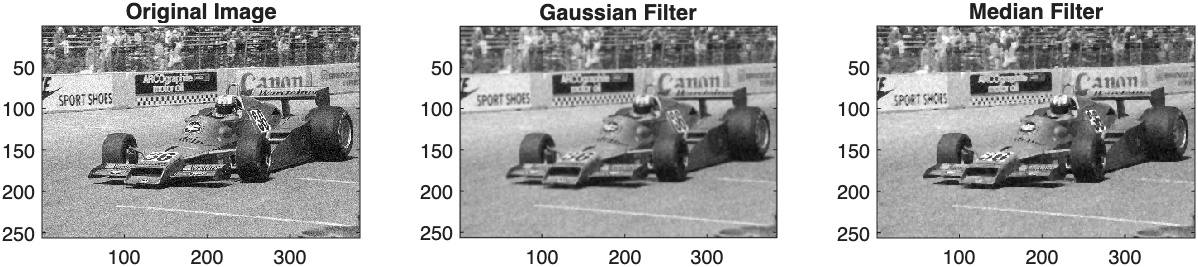
\includegraphics[width=0.8\textwidth]{../Figure_17.png}
    \caption{Noise1 with Additive White Gaussian Noise}
    \label{fig17}
\end{figure}

\begin{figure}[H]
    \centering
    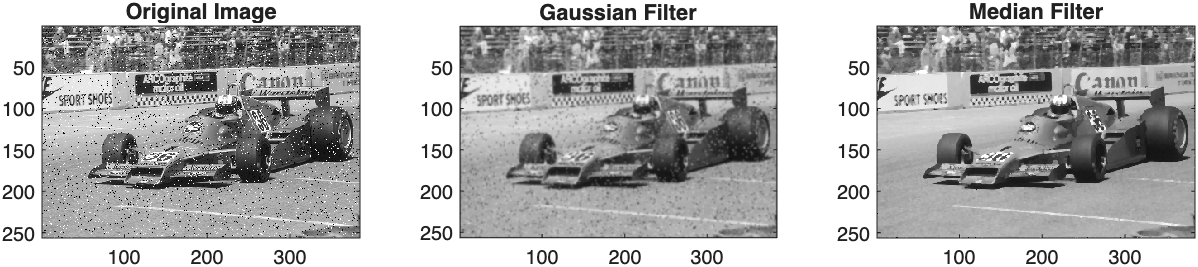
\includegraphics[width=0.8\textwidth]{../Figure_18.png}
    \caption{Noise2 with Salt and Pepper noise}
    \label{fig18}
\end{figure}


The filters in Fig. \ref{fig17} with additive white Gaussian noise both smooth out the image.
The Gaussian filter smooths the image at a stronger degree where every outline of a shape is clear.
The median filter, however, is more pixelated compared to the Gaussian filter.
In both images, differences between the most intense black and white pixels appears to be smaller. 

The "salt and pepper" noise in Fig. \ref{fig18} covers the image with black and white pixels. 
The median filter does a good job at smoothing the image and making the features appear clearer.
However, when zooming in, the car and other objects are distorted with "filler" pixels.
Additionally, the Gaussian filter morphs the dots to gray pixels that are still visible but try to blend in with the picture.

\section{Image Sharpening}
The provided equation from the problem statement,
\begin{equation}
    g(i, j) = \alpha f(i, j) - \beta [f(i, j) ** h(i, j)]
\end{equation}

can be translated into the frequency domain:
\begin{equation}
    G(w_1, w_2) = \alpha F(w_1, w_2) - \beta [F(w_1, w_2) \mathord{\cdot} H(w_1, w_2)]
\end{equation}

\begin{equation}
    G(w_1, w_2) = F(w_1, w_2)(\alpha - \beta H(w_1, w_2))
\end{equation}

\begin{equation}
    \frac{G(w_1, w_2)}{F(w_1, w_2)} = \alpha - \beta H(w_1, w_2)
\end{equation}

\begin{figure}[H]
    \centering
    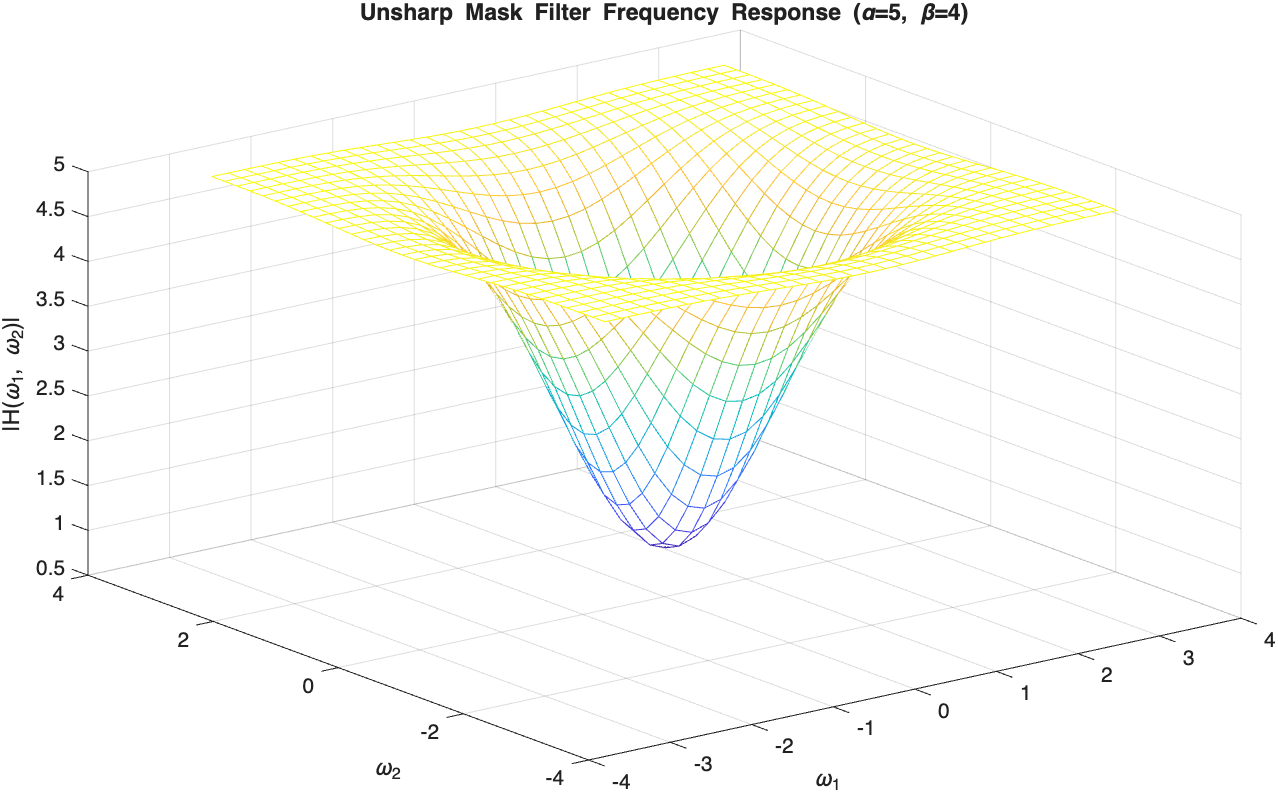
\includegraphics[width=0.8\textwidth]{../Figure_19.png}
    \caption{Unsharp Magnitude Response}
    \label{fig19}
\end{figure}

The plot in Fig. \ref{fig19} is similar to the provided plots in Figure 16.10 of the problem statement in shape. 
While Fig. \ref{fig19} does not have hyperbolic paraboloidic tendencies with curves near the borders of the range, the general structure with a peak at the origin is similar.
Specifically, Fig. \ref{fig19} behaves like Figure 16.10b, where the function is inverted along the z-axis.

\begin{figure}[H]
    \centering
    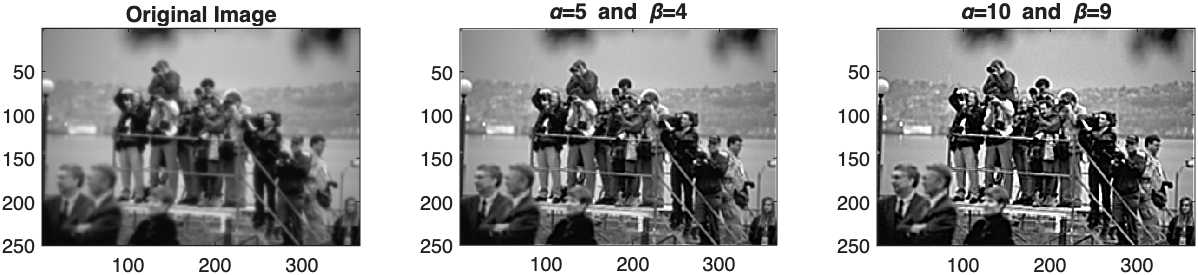
\includegraphics[width=0.8\textwidth]{../Figure_20.png}
    \caption{Processed Blur Images}
\end{figure}

The sharp contrast with the higher values of $\alpha$ and $\beta$ outline the objects to present a clearer picture.
However, with higher values, the image might be oversaturated.
Moreover, the lighter pixels in the image with higher pixels intensify and give the picture an unnatural appearance.
Whereas, the lower values provide a more real, filtered version of the blurred image.  

\end{document}
